\clearpage
\section{移动相机下的柱脚遮蔽}

一根宽 12 厘米的方柱立在地面上，右边的柱脚和左边的箱角都挡住了一部分环境光。旧图中，几条灰带像扇骨一样从柱脚伸出。移动相机时灰带也会转。两张图取自同一台相机、同一盏环境光，显示的是着色器写下的可见度。白色是 1，灰色越深，能照到这片地面的环境光越少。

\begin{center}
\panelimage{.48\linewidth}{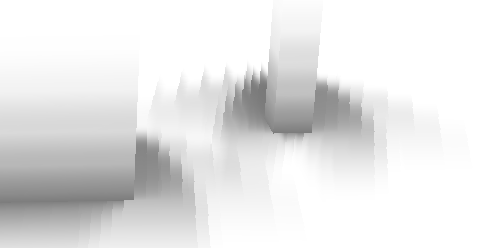
\includegraphics[width=\linewidth]{../../../output/validation/gtao-motion/forge-before/post-detail.png}}{修改前。柱脚两边能分辨出几条窄带。}\hfill
\panelimage{.48\linewidth}{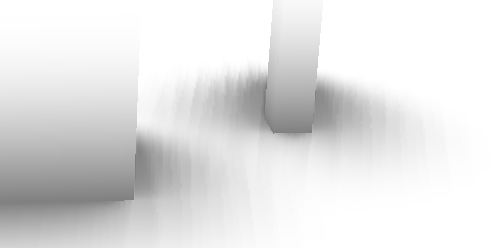
\includegraphics[width=\linewidth]{../../../output/validation/gtao-motion/forge-after/post-detail.png}}{修改后。箱角和柱脚各自保留了遮蔽。}
\end{center}

原着色器在每个像素上都查同样的四个方向。遇到远处的轮廓时，它先按距离减弱轮廓的角度，再拿这个角度估整段遮挡。现在每次遇到新轮廓，只给它额外挡住的那段方向乘距离权重。相邻四个像素也会略微转动各自的截面，再从周围的同一平面取平均。每个像素仍最多查 64 次表面。第二次计算需用一张每像素 4 字节的可见度图，1920$\times$1080 共用 7.91\,MiB。

在 $320\times180$ 的 Vulkan 回归中，相机向右移动 1.8 米，经过 13 个机位。每帧重新找回箱前和柱前距接触线 2 至 10 厘米的地面点。参考值来自每点 8192 条半球射线，使用与着色器相同的 65 厘米半径和距离衰减。下表的误差和逐帧差都是 0 到 1 之间的可见度差。TAA 开启时按面板的固定像素读最终颜色，单独读当前帧的遮蔽时则使用当帧实际的采样位置。

{\smalltable\noindent\begin{tabularx}{\linewidth}{@{}Xrr@{}}\toprule
透视相机连续移动 & 旧版 & 新版\\\midrule
箱脚与参考值的平均绝对误差，关闭 TAA & 0.03207 & 0.01512\\
柱脚与参考值的平均绝对误差，关闭 TAA & 0.07100 & 0.04154\\
柱脚相邻两帧的平均差，开启 TAA & 0.02211 & 0.01591\\
柱脚相邻两帧的平均差，关闭 TAA & 0.01640 & 0.01565\\\bottomrule
\end{tabularx}}

另用正式游戏窗口输出 $1920\times1080$，取左、中、右三个机位的第 8 帧。在方柱周围四条圆上与射线参考比较，中间机位可见的 666 个点的平均误差从 0.123 降到 0.101。射线能找到柱子背面，GTAO 只能读画面里看得见的第一层表面，这部分差别仍在。正交相机的回归中，柱脚逐帧差从 0.01283 升到 0.01434，虽然与参考的平均误差降低，运动时仍有改善余地。

两份正式帧都在 RTX 5070 Ti Laptop GPU 上以 RenderDoc 1.47 回放。预热一次后，读取 11 次 GPU 事件时间的中位数。旧版事件 85 用 1.312\,ms，新版事件 85、96 合计 2.045\,ms，合成间接光从事件 97 移到 108。几何绘制数量相同。这次没有单独计 CPU 提交时间。下一次可试用较小、连续存储的深度图做轮廓搜索，在这三个机位复测读取成本和柱脚误差。截图、逐次耗时和复现入口见 \path{output/validation/gtao-motion/}。
